\subsection{Data Description and Task DNA Source}We extract task statements and task ratings for SOC 15-1252.00 from the O*NET 30.1 text database and calculate task weights based on Importance (IM) and Frequency of Task (FT) ratings. \cite{onet2025database}\begin{table}[htbp]
\centering
\caption{Data Sources and Variables for Task DNA}
\label{tab:data_sources_task_dna}
\begin{tabular}{@{}p{3.4cm} p{7.4cm} p{3.2cm}@{}}
\toprule
Variable/Data & Description & Source \\
\midrule
O*NET Task Statements & Task text and identifiers for SOC 15-1252.00 & O*NET 30.1 Database\newline \cite{onet2025database} \\
O*NET Task Ratings (IM, FT) & Importance and Frequency ratings used to calculate task weights & O*NET 30.1 Database\newline \cite{onet2025database} \\
Task DNA CSV & Processed task table containing IM, FR, weights, and rule-based s/c & Derived from O*NET 30.1\newline \cite{onet2025database} \\
\bottomrule
\end{tabular}
\end{table}\begin{figure}[htbp]
\centering
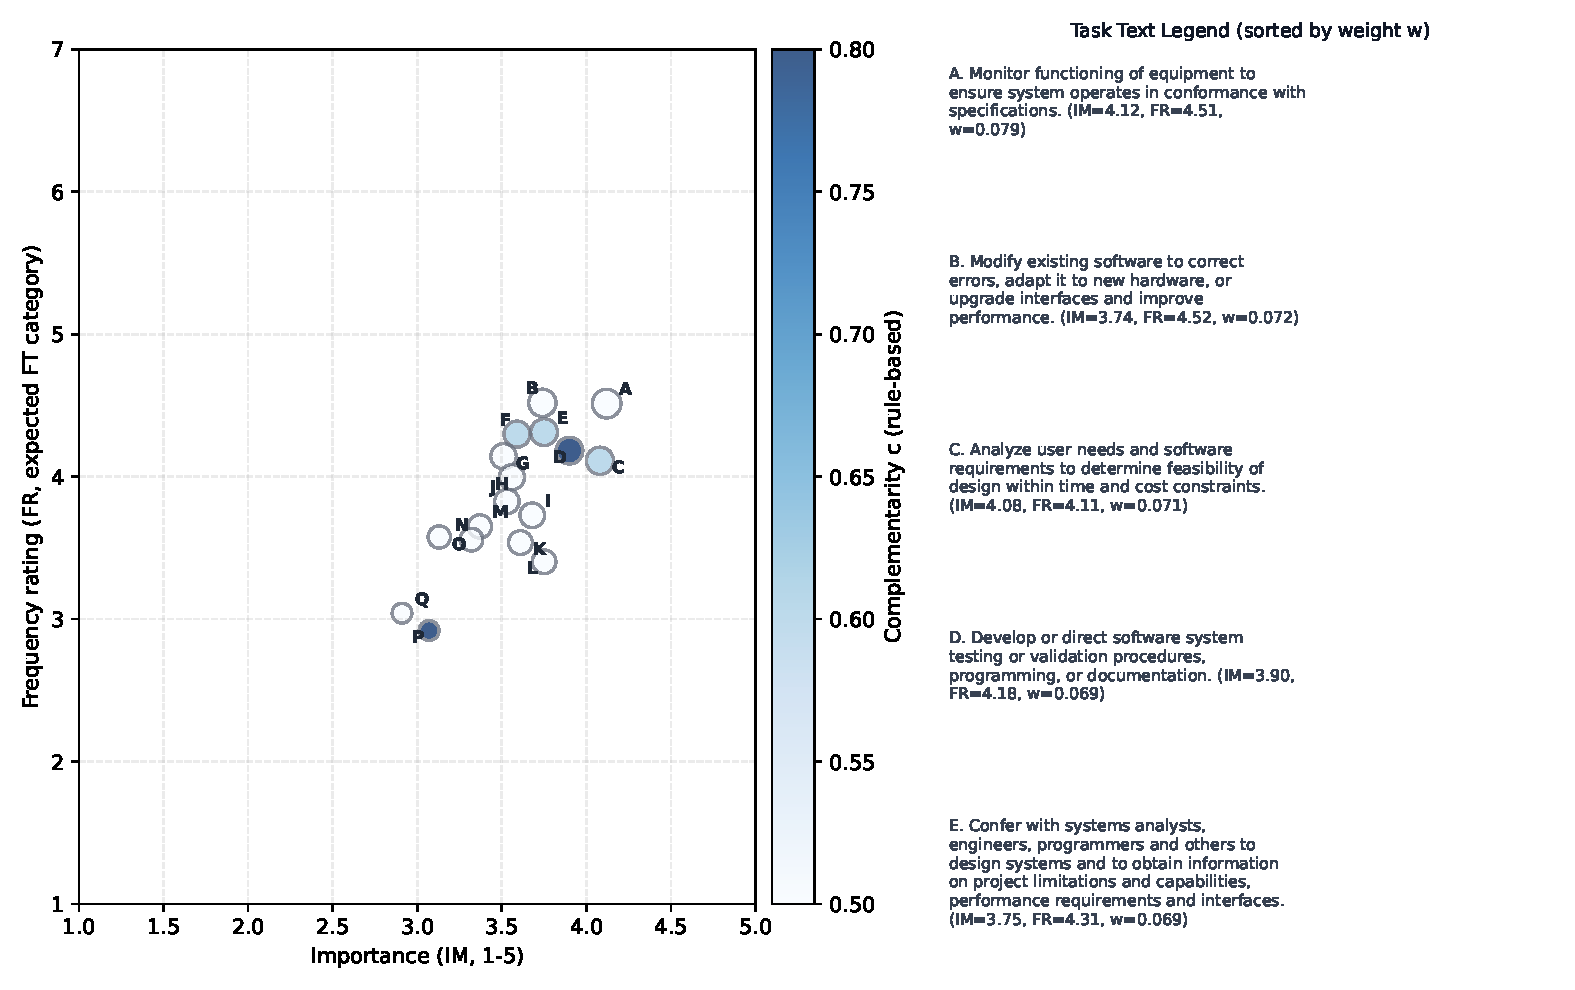
\includegraphics[width=0.82\textwidth]{figures/task_dna_15-1252_weights.pdf}
\caption{Task-level IM--FR exposure for software developers (SOC 15-1252.00). Bubble size encodes the normalized task weight $w$, color encodes rule-based complementarity $c$, and edge thickness reflects rule-based substitutability $s$. Letter labels map to task text in the legend panel.}
\label{fig:task_dna_im_fr}
\end{figure}
